\documentclass[12pt,a4paper]{article}

% Paquetes básicos
\usepackage[utf8]{inputenc}
\usepackage[T1]{fontenc}
\usepackage[spanish]{babel}
\usepackage{amsmath, amssymb}
\usepackage{siunitx} % Ángulos
\usepackage{graphicx}
\usepackage{float}
\usepackage{geometry}
\usepackage{xcolor}
\geometry{margin=2.5cm}
\usepackage{array}
\usepackage{longtable}
\usepackage{hyperref}
\usepackage{caption}
\usepackage{subcaption}
\usepackage{setspace}
\usepackage{multirow}
\usepackage{minted}  % Códigos
\usepackage{gensymb} % Grados: "°"
\usepackage[backend=biber, style=ieee]{biblatex}
\usepackage{csquotes}
\usepackage{booktabs}
\addbibresource{Bibliografía.bib}
\graphicspath{{Figuras/}}
\onehalfspacing
\hypersetup{
    colorlinks  = true,
    linkcolor   = blue,    
    citecolor   = blue,
    urlcolor    = blue,
    filecolor   = blue
}


\begin{document}       
\renewcommand{\figureautorefname}{Fig.}
\renewcommand{\tableautorefname}{Tab.}
\renewcommand{\equationautorefname}{Ec.}


% Carátula personalizada
\begin{titlepage}
    \centering
    
\includegraphics[width=0.7\textwidth]{Marvell Logo.png}\\[1.5cm]

    {\Large \textbf{PROGRAMA DE FORMACIÓN MARVELL} \\[0.5cm]}
    {\Large Diseño Digital para Sistemas DSP} \\[0.5cm]

    \rule{\textwidth}{0.5pt} \\[0.5cm]
    {\Large \textbf{Ejercicios Módulo 5: Circuitos Aritméticos II} \\[0.3cm]}
    \rule{\textwidth}{0.5pt} \\[1cm]
    
\vfill
\begin{tabular}{l l}
    \textbf{Profesor:} & Del Barco, Martín.\\
    \\[0.5cm]
    \textbf{Alumnos:} & Monja, Ernesto Joaquín\\
                      & Zúñiga, Guillermo Rubén Darío\\
\end{tabular} \\[5cm]
\vfill
{\centering Año 2026 \par}

\end{titlepage}



% Índice
\tableofcontents
\newpage



\section{Introducción}                                              \label{sec_1}
El presente trabajo práctico aborda el diseño e implementación en \textit{SystemVerilog} de algoritmos iterativos fundamentales para el procesamiento digital de señales (\textit{DSP}), centrándose específicamente en las arquitecturas \textit{CORDIC} y métodos como \textit{Newton-Raphson}. A través del desarrollo de módulos operando estrictamente en aritmética de punto fijo, se exploran los modos de rotación y vectorización para el cálculo eficiente de funciones trigonométricas, magnitudes y fases, prescindiendo de multiplicadores dedicados y memorias de gran escala. Asimismo, el estudio analiza empíricamente los compromisos espacio-temporales (\textit{PPA}) al contrastar enfoques secuenciales (\textit{folded}) frente a topologías segmentadas de alta velocidad (\textit{pipeline}), validando la precisión algorítmica y la correcta latencia de cada \textit{datapath} mediante simulaciones \textit{RTL} e inspección de formas de onda.



\section{Desarrollo}                                                \label{sec_2}
\subsection{\textit{CORDIC} iterativo en \textit{Verilog}}          \label{sec_2.1}
Para este ejercicio se implementó una arquitectura \textit{CORDIC} tipo \textit{folded} orientada al cálculo del seno y coseno de un ángulo entrante. El \textit{HW} se diseñó operando íntegramente en punto fijo con formato $S(16,14)$, lo que destina un bit para el signo, un bit entero y catorce bits fraccionales.

El \textit{datapath} se compone de un par de \textit{shifters} aritméticos ($> \, > \, >$) y sumadores/restadores, controlados por una máquina de estados finitos (\textit{FSM}) encargada de secuenciar el cálculo. Al iniciar la \textit{FSM}, la variable $x_{0}$ se inicializa en un valor pre-escalado de aproximadamente $0.60725$ (representado como $9949$ en cuantización $S(16,14)$). Esto evita un escalado posterior del resultado.

Durante el estado de \textit{ITER}, el módulo ejecuta un total de $14$ iteraciones a lo largo de $14$ ciclos de reloj. En cada ciclo, el signo de $z$ dictamina el sentido de la rotación (determina $d_{i}$) y actualiza $x$, $y$ y $z$ utilizando los valores precalculados de $\arctan(2^{-i})$ leídos directamente de una matriz combinacional que actúa como \textit{ROM}.

En el banco de pruebas se evaluaron los ángulos en el primer cuadrante especificados por la consigna: $\pi/6$, $\pi/4$ y $\pi/3$. Al analizar las formas de onda (ver \autoref{fig:fig_1}), se observa claramente el retardo de $14$ ciclos por cada muestra introducida, validando que el diseño intercambia área por latencia (característica definitoria de la arquitectura \textit{folded}) para evitar la instanciación de multiplicadores dedicados. Asimismo, la correcta convergencia del algoritmo se comprueba en la salida de consola (ver \autoref{fig:fig_2}), donde los valores de seno y coseno coinciden con la precisión esperada para el formato numérico utilizado.
\begin{figure}[H]
    \centering
    
\includegraphics[width=1.05\textwidth]{Figura 1.png}
    \caption{Formas de onda de la simulación del módulo \textit{CORDIC}.}
    \label{fig:fig_1}
\end{figure}

\begin{figure}[H]
    \centering
    
\includegraphics[width=0.55\textwidth]{Figura 2.png}
    \caption{Salida de la consola del simulador detallando los resultados del ángulo evaluado.}
    \label{fig:fig_2}
\end{figure}



\subsection{\emph{CORDIC} Pipeline}         \label{sec_2.2}
En esta sección, se diseñó el mismo algoritmo que en el caso anterior pero en una estructura de mínima latencia, donde se replicaron los bloques de iteración en cascada y se separaron con registros enmedio. El esquema de esta estrategia se muestra en la \autoref{fig:esq_pipeline}.
\begin{figure}[H]
    \centering
    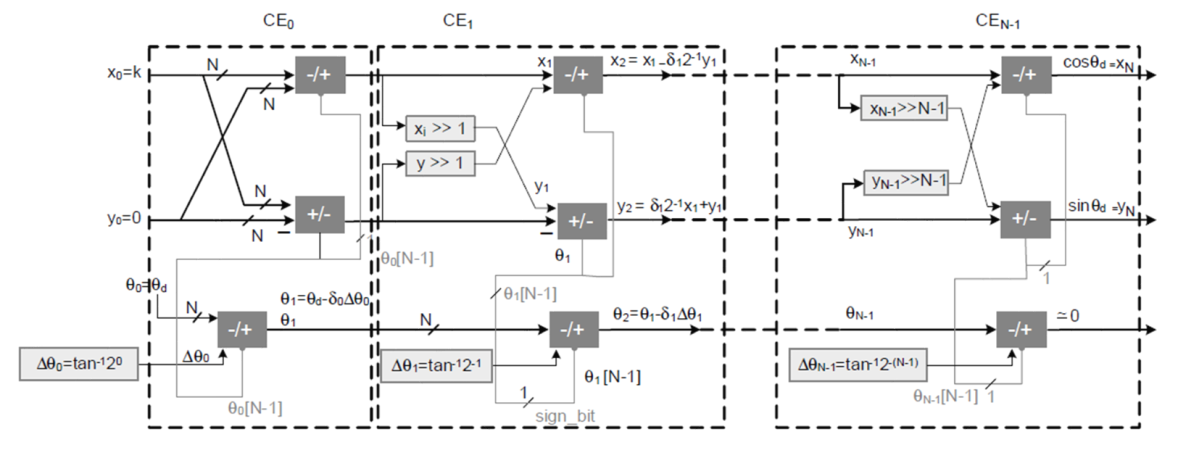
\includegraphics[width=0.9\linewidth]{Figuras/esq_pipeline.png}
    \caption{Esquemático del CORDIC pipeline.}
    \label{fig:esq_pipeline}
\end{figure}

Esto resultaría en una latencia de $N_{iter}$ ciclos de reloj para observar el dato a la salida, pero solo al inicio del stream de datos a la entrada, luego la latencia es de 1. En cuanto al throughput, este diseño permitiría entregar 1 muestra por ciclo.

Se diseñó en Verilog esta arquitectura con datos en S(16,14), resultando en 14 etapas, con el objetivo de procesar ángulos de entrada en radianes entre $-\pi/2$ y $\pi/2$. El testbench desarrollado estimula la entrada $z_i$ con $0$, $\pi/2$, $-\pi/2$ y valores aleatorios positivos y negativos generados en Python, con $x_i = 1/K$ ya que el algoritmo escala implícitamente la salida por la constante $K$. El resultado se observa en las formas de onda de la \autoref{fig:sim_pipeline}. Se puede comprobar que efectivamente el sistema tarda 14 ciclos en entregar los valores de salida, luego el stream es continuo.
\begin{figure}[H]
    \centering
    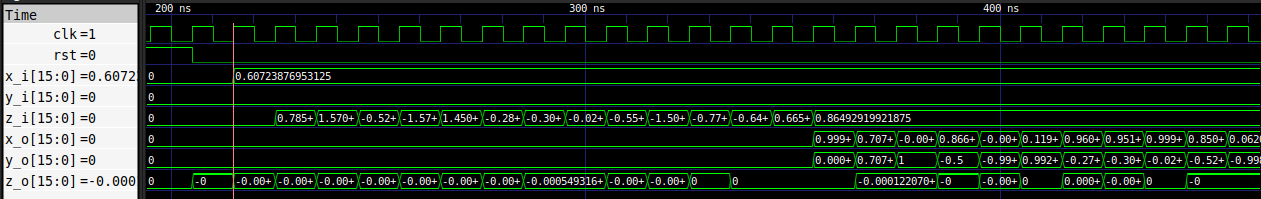
\includegraphics[width=\linewidth]{Figuras/sim_pipeline.png}
    \caption{Formas de onda en el diseño con pipeline.}
    \label{fig:sim_pipeline}
\end{figure}

Cabe destacar que este diseño no escala las entradas para aprovechar el máximo rango dinámico del punto fijo, sin embargo, se observó gran similitud con los resultados obtenidos en punto flotante.

Finalmente, se comparó el area y el número de compuertas entre la estructura folded y con pipeline utilizando Yosys. La frecuencia máxima para el reloj es la misma, ya que un bloque de iteración se encuentra entre dos registros en ambos casos, pero la frecuencia máxima del dato es diferente como se vio anteriormente. La comparación se resume en la \autoref{tab:folded_pipeline}, dada $N_{iter}$ iteraciones. Se concluye con estos datos entonces que la arquitectura pipeline es más rápida pero ocupa más área, ya que replica varias veces el bloque que utiliza el folded.
\begin{table}[H]
    \centering
    \begin{tabular}{c|cc} \toprule
        \textbf{Arquitectura}                  & \textbf{Folded} & \textbf{Pipeline} \\ \midrule
        \textbf{Nro. de celdas}                & 674             & 4806              \\
        \textbf{Área del chip} [\textmu m$^2$] & 7737            & 50278             \\
        \textbf{Throughput} [muestras/seg.]    & $1/N_{iter}$    & 1 (en régimen)    \\
        \textbf{Latencia}                      & N               & N                 \\ \bottomrule % Revisar
    \end{tabular}
    \caption{Comparación entre CORDIC folded y pipeline.}
    \label{tab:folded_pipeline}
\end{table}



\subsection{\textit{CORDIC Vectoring} para magnitud}                \label{sec_2.3}
En este ejercicio se implementó el algoritmo \textit{CORDIC} configurado en modo \textit{vectoring} para obtener la magnitud $R = \sqrt{x^2 + y^2}$ y la fase $\varphi = \arctan(y/x)$ de un vector bidimensional de entrada.

A diferencia del modo rotación, la \textit{FSM} ajusta la regla de decisión en cada iteración según el signo del registro $y$: $d_{i} = -signo(y_{i})$. Este procedimiento reduce la componente cuadratura a cero mientras acumula el ángulo total rotado en el registro $z$.

Para asegurar el correcto funcionamiento en los cuatro cuadrantes y evitar la divergencia del algoritmo ante ángulos $|\varphi| > 99.88^\circ$, se incorporó una etapa de pre-rotación combinacional. Si la coordenada $x < 0$ (Cuadrantes \textit{II} y \textit{III}), se invierten los signos de $x$ e $y$, y el registro $z$ se inicializa en $+\pi$ o $-\pi$ según corresponda.


\subsubsection{Análisis de Formatos Numéricos y Precisión}
Para representar la fase en todo el rango $[-\pi, \pi]$ sin caer en \textit{overflow} con palabras de $16$ bits, el registro de ángulo $z$ y la \textit{ROM} de $\arctan(2^{-i})$ se codificaron en formato $S(16,13)$, permitiendo valores de hasta $\pm 4.0$. Por su parte, las entradas y la magnitud resultante operan en formato $S(16,15)$.

En la \autoref{fig:fig_3} se presentan los resultados obtenidos de la simulación para vectores en los cuatro cuadrantes. Como se observa en la \autoref{fig:fig_4}, el circuito procesa cada muestra con una latencia fija de $16$ ciclos. El error relativo de la magnitud $R$ se mantiene por debajo del $\approx 0.05 \, [\%]$, independientemente del cuadrante evaluado.
\begin{figure}[H]
    \centering
    
\includegraphics[width=0.85\textwidth]{Figura 3.png} % consola
    \caption{Resultados obtenidos por consola para vectores de prueba en los cuatro cuadrantes.}
    \label{fig:fig_3}
\end{figure}

\begin{figure}[H]
    \centering
    
\includegraphics[width=1.05\textwidth]{Figura 4.png} % ondas
    \caption{Formas de onda mostrando la convergencia del registro $y$ a cero y el cálculo de $R$ y $\varphi$.}
    \label{fig:fig_4}
\end{figure}


\subsubsection{Comparación frente a Implementación Directa con Multiplicador y ROM}
Frente a una arquitectura tradicional de fuerza bruta que calcula $R = \sqrt{x^2 + y^2}$ mediante multiplicadores ($x^2, y^2$), un bloque de raíz cuadrada (por ejemplo: \textit{coredic/CORDIC} dedicado o aproximación por polinomio) y una memoria Look-Up Table (\textit{LUT}) bi-dimensional para $\arctan(y/x)$, la solución \textit{CORDIC} presenta ventajas determinantes:
\begin{itemize}
    \item \underline{Ahorro masivo de área:} Evita bloques \textit{DSP} dedicados y memorias \textit{ROM} de gran escala, requiriendo únicamente sumadores, acumuladores y desplazadores aritméticos (\textit{shifters}).
    \item \underline{Cálculo simultáneo:} Resuelve magnitud y fase de manera concurrente en la misma secuencia iterativa.
\end{itemize}



\subsection{Newton-Raphson para \textit{1/x}}                       \label{sec_2.4}
En esta sección se estudió la arquitectura del divisor Newton-Raphson para realizar divisiones eficientes. La idea es encontrar el resultado de un valor $1/a$ con aproximaciones sucesivas, realizando

\begin{equation}
    y_n = y_{n-1} (2 - a\cdot y_n)
\end{equation}

\noindent
donde se comienza con un valor inicial $y_o$ hasta obtener el valor final $y_N$ luego de $N$ iteraciones.
En Verilog se realizó el diseño, tomando como referencia el esquema de la \autoref{fig:esq_nr}. Se supuso $a \in [0.5,1)$ y una LUT de 8 valores iniciales. Luego, se fue observando en la forma de onda la precisión del resultado con el valor real. 

\begin{figure}[H]
    \centering
    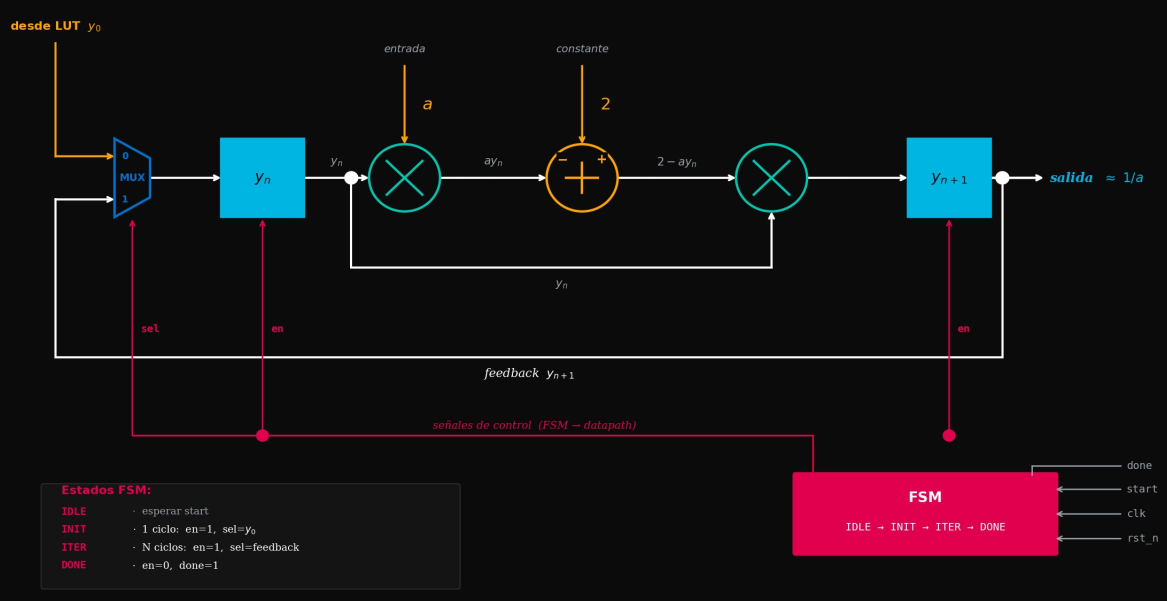
\includegraphics[width=\textwidth]{Figuras/esq_nr.png} % ondas
    \caption{Esquema propuesto del divisor Newton-Raphson.}
    \label{fig:esq_nr}
\end{figure}

En la \autoref{fig:sim_nr} se puede ver la salida del sistema \texttt{y\_o} cuando la bandera \texttt{done} se levanta (se completó la operación) luego de 7 iteraciones, para $y_{inicial} = 0.1$. A simple vista se observa una precisión de 2 dígitos decimales, luego si se ve a nivel de bits, se obtiene una precisión de hasta 10 dígitos.

\begin{figure}[H]
    \centering
    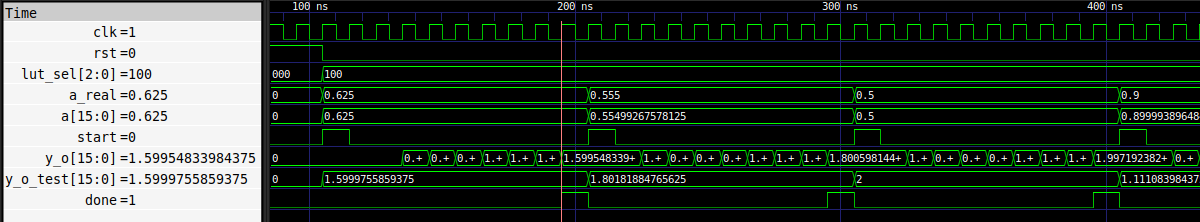
\includegraphics[width=\textwidth]{Figuras/sim_nr.png} % ondas
    \caption{Formas de onda obtenidas con $a = 0.625$, $0.555$ y $0.5$. $y_{inicial} = 0.1$}
    \label{fig:sim_nr}
\end{figure}

\begin{figure}[H]
    \centering
    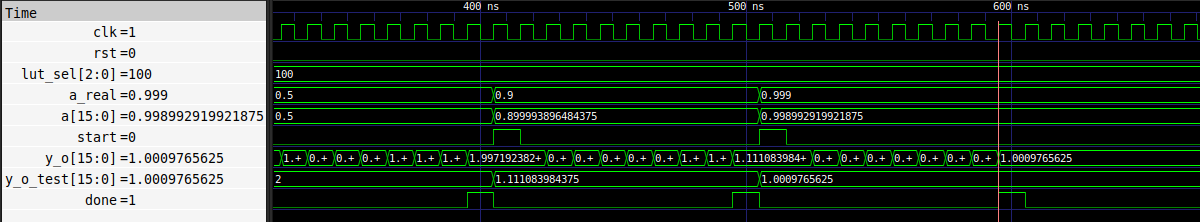
\includegraphics[width=\textwidth]{Figuras/sim_nr2.png} % ondas
    \caption{Formas de onda obtenidas con $a = 0.9$ y $0.999$. $y_{inicial} = 0.1$}
    \label{fig:sim_nr2}
\end{figure}

La \autoref{tab:nr} muestra cómo evoluciona el error del sistema a medida que aumentan las iteraciones. En un escenario ideal, se esperaría que en 3 o 4 iteraciones el error ya sea imperceptible, sin embargo, la elección en este caso del valor inicial y los errores de cuantización generaron un peso importante sobre la precisión final. De todas formas, se pudo concluir que el número de bits correctos aumenta cuadráticamente con cada iteración.

\begin{table}[H]
    \centering
    \begin{tabular}{c|ccc} \toprule
        \textbf{Iteración} & \textbf{Obtenido} & \textbf{Error} [\%] & \shortstack{\textbf{Nro. de bits} \\ \textbf{correctos}} \\ \midrule
        1 & $0.1937255859$ & $87.9$ & 1 \\
        2 & $0.3639526367$ & $77.2$ & 1 \\
        3 & $0.6451416016$ & $59.7$ & 1 \\
        4 & $1.0301513672$ & $35.6$ & 2 \\
        5 & $1.3970336914$ & $12.7$ & 2 \\
        6 & $1.5742187500$ & $1.61$ & 6 \\
        7 & $1.5995483398$ & $0.0282$ & 10 \\ \bottomrule
    \end{tabular}
    \caption{Métricas obtenidas para $1/0.625 = 1.6$. $y_{inicial} = 0.1$}
    \label{tab:nr}
\end{table}

\section{Conclusiones}                                              \label{sec_3}
Se demostró entonces que las arquitecturas iterativas en punto fijo permitieron implementar funciones matemáticas complejas en hardware sin recurrir a multiplicadores dedicados o memorias extensas. En las implementaciones del CORDIC, el modo rotación calculó seno y coseno en 14 iteraciones, mientras que el modo vectoring resolvió magnitud y fase simultáneamente en los cuatro cuadrantes gracias a la pre-rotación, con un error relativo inferior al 0.05\%. La comparación en la síntesis evidenció que el pipeline multiplica el área 6 veces en comparación del folded (4806 vs. 674 celdas), con la ventaja de aumentar el throughput. Por último, el divisor Newton-Raphson alcanzó 10 bits correctos tras 7 iteraciones, confirmando la convergencia cuadrática teórica.



\newpage
\nocite{*}
\printbibliography[heading=bibintoc, title={4. \ Referencias}]

\end{document}